\section{Fluxo de desenvolvimento}\label{sec:figs}

Para desenvolver em um repositório precisamos usar uma branch, ou ramificação no português. Por padrão, todo repositório gerado pelo template possui uma branch chamada main. Essa branch possui uma configuração automática onde toda vez que é feita uma nova versão dela é gerada uma nova release no repositório. A image~\ref{fig:image05} mostra a ultima versao do template na plataforma do Github.

\begin{figure}[ht]
	\centering
	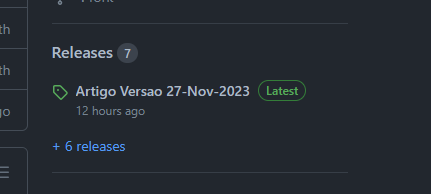
\includegraphics[width=.5\textwidth]{./images/image06.png}
	\caption{Ultima release}
	\label{fig:image06}
\end{figure}


Ao clicar na release, vai aparecer as informações da data da release junto com o arquivo em pdf (imagem~\ref{fig:image07}). isso permitirá que as pessoas com acesso ao repositório peguem a ultima versão do pdf sem a necessidade de abrir o latex.

\begin{figure}[ht]
	\centering
	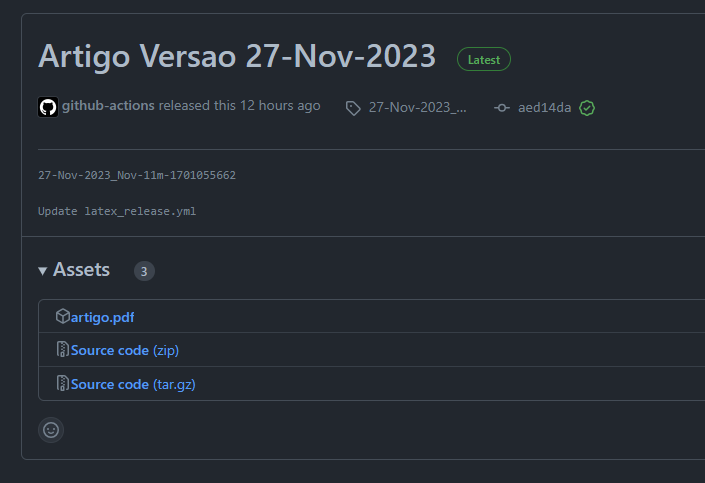
\includegraphics[width=.5\textwidth]{./images/image07.png}
	\caption{Detalhes da ultima release}
	\label{fig:image07}
\end{figure}

Para orientadores e outros envolvidos que não possuem o interesse ou a permissão para alterar o texto é uma funcionalidade bastante útil, pois evita de precisar gerar um novo pdf a cada acesso e mantém a confiabilidade da versão do tcc.
É possível ver as releases anteriores do tcc também. basta acessar a aba releases (imagem~\ref{fig:image08}), na tela da ultima release.


\begin{figure}[ht]
	\centering
	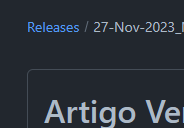
\includegraphics[width=.5\textwidth]{./images/image08.png}
	\caption{Aba releases}
	\label{fig:image08}
\end{figure}


\begin{figure}[ht]
	\centering
	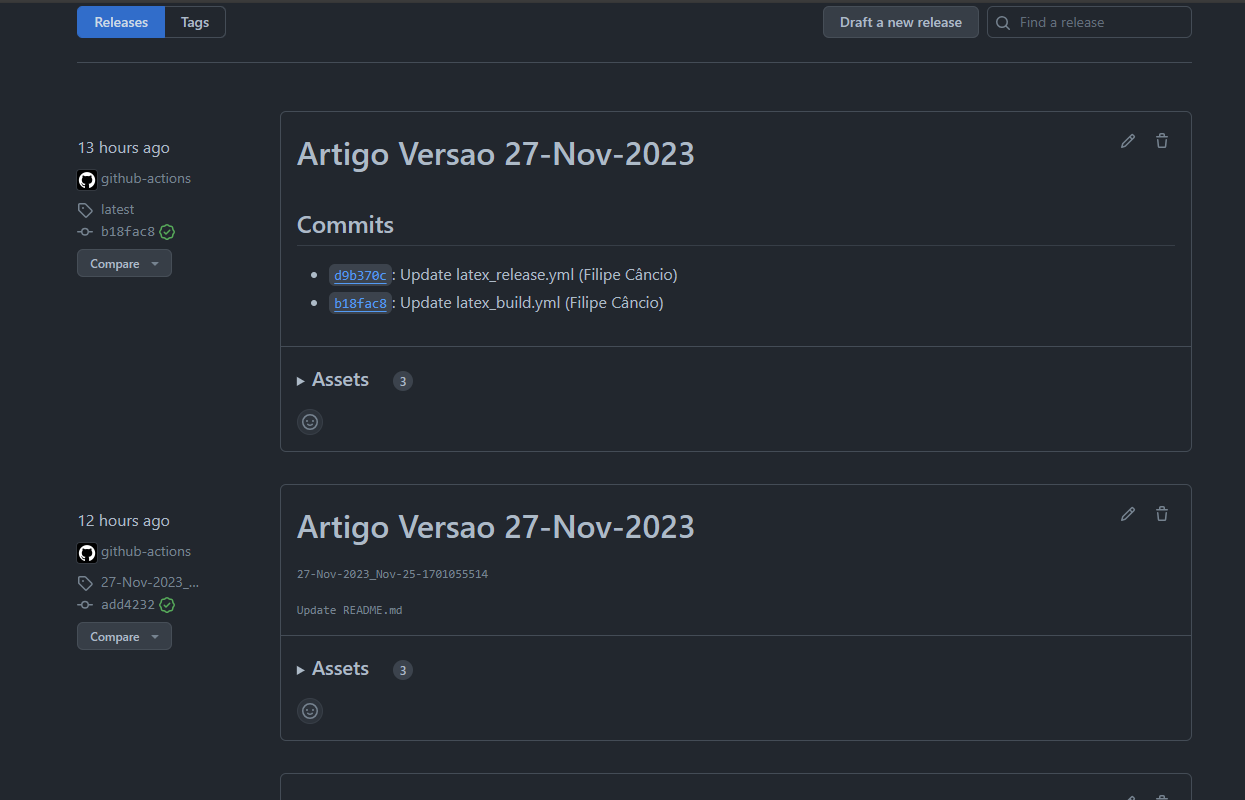
\includegraphics[width=.5\textwidth]{./images/image09.png}
	\caption{Lista de releases}
	\label{fig:image09}
\end{figure}

A utilização dessa funcionalidade permite ao autor a simples necessidade de subir o projeto para o repositório para cada versãoo ou se preferir alterar arquivos na própria plataforma.

\subsection{Boas práticas de desenvolvimento}

Por mais comum que seja, editar na ramificação main, não é o ideal. No caso do projeto atual, o autor pode acabar gerando um número excessivo de release que com o tempo não farão muito sentido, será impraticável saber qual a release certa para cada alinhamento feito com o orientador. Para isso é recomendado que o autor crie novas ramificações para o desenvolvimento do artigo, deixando a branch main somente para as versões finais, ou de revisão do orientador.
Ao criar uma nova ramificação, ainda assim, é gerado um novo pdf a cada commit. O autor pode verificar os pdfs gerados na aba Actions do repositório (imagem~\ref{fig:image10}). Lá cada versão terá o nome da mensagem de commit e terá por anexo o pdf gerado (imagem~\ref{fig:image11}). Isso permitira um fluxo de desenvolvimento mais limpo e fácil de validar correções.



\begin{figure}[ht]
	\centering
	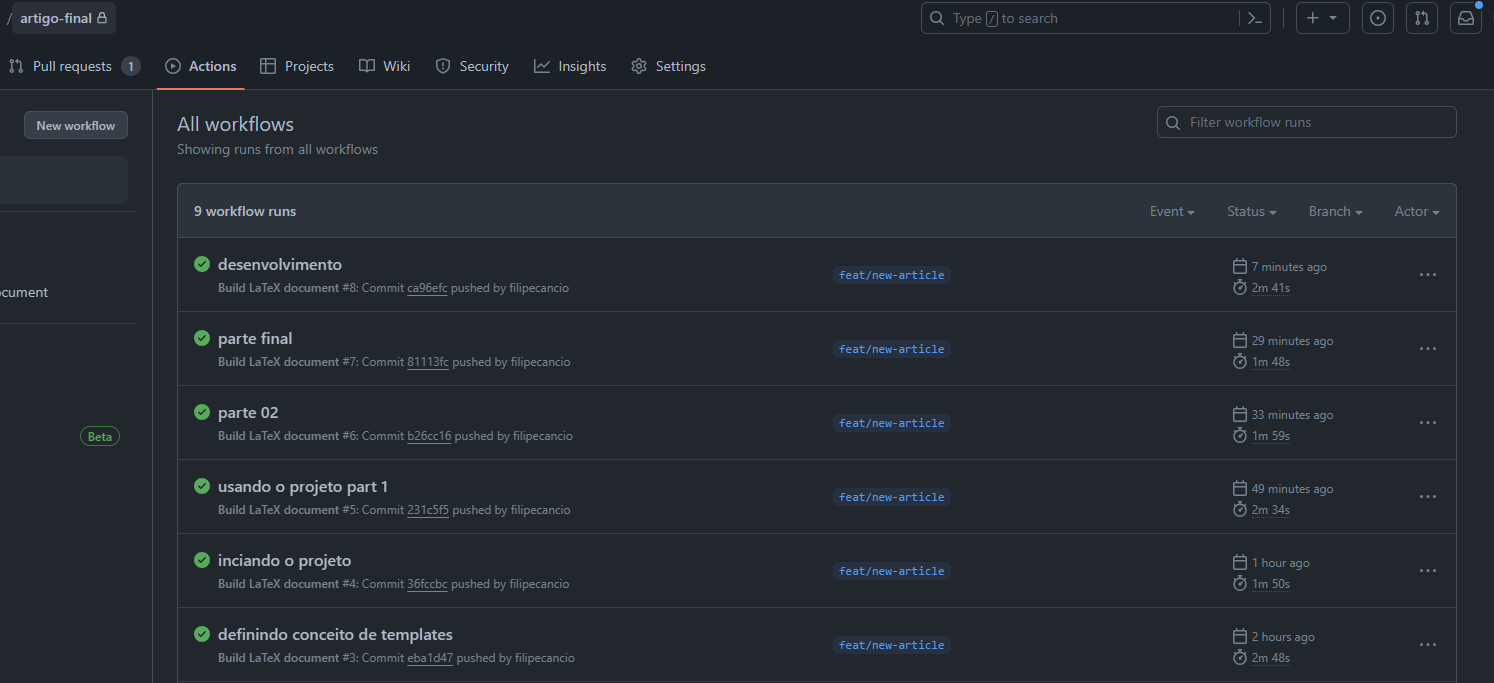
\includegraphics[width=.5\textwidth]{./images/image10.png}
	\caption{Aba actions}
	\label{fig:image10}
\end{figure}


\begin{figure}[ht]
	\centering
	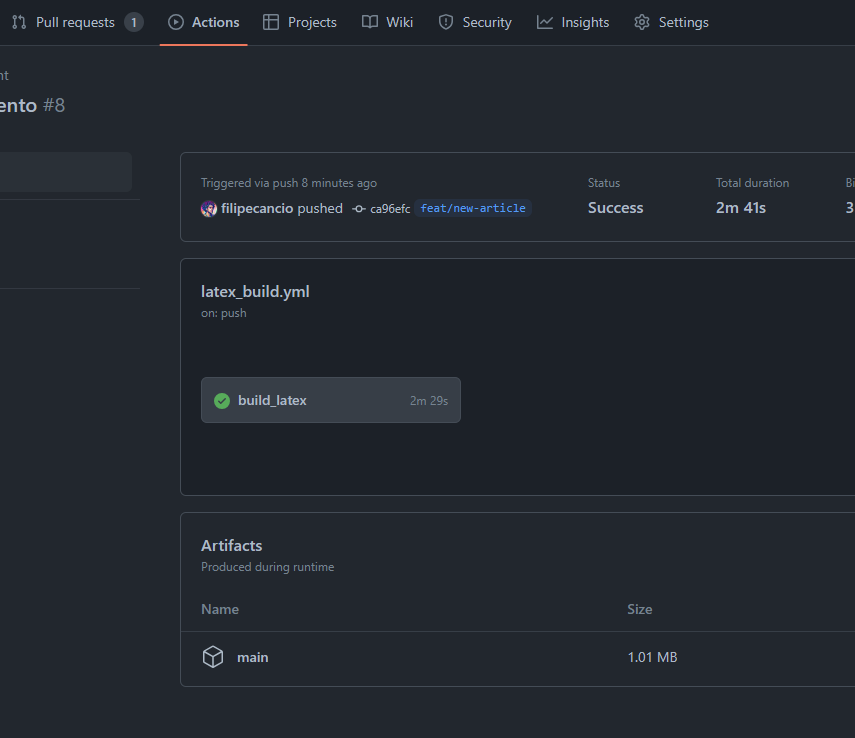
\includegraphics[width=.5\textwidth]{./images/image11.png}
	\caption{Action aberta}
	\label{fig:image11}
\end{figure}

Neste projeto não é definido um modelo fixo de fluxo de desenvolvimento, apenas a utilização ou não da branch main. Mas deixa um espaço aberto para os mais variado usos das ferramentas do github para o desenvolvimento de artigos.